\chapter{De-Entanglement by Divergence}

section{Visual Question Answering}

Visual Question Answering (VQA) involves answering a natural language query about an image. Questions can be arbitrary and they encompass many sub-problems in computer vision: (1) Object recognition %- What is in the given image? 
(2) Object detection %- Are there any cats in the image? 
(3) Attribute classification %- What color is the cat if present ? 
(4) Scene classification %- Is it raining? 
(5) Counting. % - How many dogs are in the image? 
VQA is characterized by wide ranging applications from helping visually impaired people through human machine interaction. It has the potential to serve as an effective media content retrieval framework. 
%VQA is a challenging task since it requires reasoning across multiple modalities. It involves additional challenges of knowledge representation and reasoning both within and across them. For example,given a picture of cat, the question ‘Is the cat black in color?’  can be answered using the visual modality once the model understands that it is to check the color of cat. The information about what to look for comes from the text modality. So in the general setting, the VQA model has to combine the information from both the modalities and reason over this combined representation. 
A primary form of implementing a VQA system would be to use a bucketing approach: by learning image and text features and fusing them to get an answer. In recent years, there have been several extensions to the trivial approach mentioned above \cite{fukui2016multimodal}; \cite{lu2016hierarchical}; \cite{yang2016stacked}; \cite{lu2015deeper} claim to learn good representations of abstract concepts needed to answer questions. However, it has been shown \cite{agrawal2017c} that most of the approaches capture surface level correlations and fail to handle unseen novel combinations during test time. 
%Recently, the ability of VQA models to handle compositionality has been greatly sought after. Few models address the inferencing and reasoning abilities of VQA models that is provided by the properties of compositionality.

In this work, we investigate approaches to improve compositionality in VQA, where we explicitly focus on learning compositionality between concepts and objects. Language and vision are inherently composite in nature. For example different questions share substructure viz \textit{Where is the dog?} and \textit{Where is the cat?} Similarly images share abstract concepts and attributes viz \textit{green pillow} and \textit{green light}. Hence it is vital not only to focus on understanding the information present across both these modalities, but also to model the abstract relationships so as to capture the unseen compositions of seen concepts at test time. Achieving this would then allow the model to generalize better by learning an inference procedure, resulting in true success on this task.

In this work, we propose \textbf{\textit{JUPITER}} - \textbf{JU}stification via \textbf{P}ointwise combination of \textbf{I}mage and \textbf{T}ext based on \textbf{E}xpected \textbf{R}ewards, is built on top of the Neural Module Networks \cite{HuARDS17}. This is motivated from our hypothesis that generating captions can provide additional information to improve VQA. Additionally, JUPITER uses Reward Augmented Maximum Likelihood \cite{RAML}, which is improves caption generation.

section{Related Work}
\noindent\textbf{Visual Question Answering}: \cite{KazemiE17} provided a strong baseline for VQA using a simple CNN-LSTM architecture, and achieved 64.6\% on the VQA 1.0 Openended QA challenge. This further proved that the dataset is biased. \cite{AishAgrawal17} introduced grounding to prevent the model from memorizing this bias. Similarly, \cite{li2018zero} used a zero-shot training approach to improve the generalizabilty of the model, and prevent the model to learn the bias. However, recently \cite{AgrawalKBP17} showed that most models degrade in performance when tested on unseen samples. In this work, we aim to tackle this lack of generalizability.
\\

\noindent\textbf{Neural Module Networks}: To the best of our knowledge, the work by authors in \cite{HuARDS17} and \cite{deepmodulenets} is the only work so far that explicitly uses a divide and conquer approach for compositionality. Natural language questions are best answered when broken down into their subparts. The authors use a similar intution and propose a modular architecture. This approach first parses the natural language question into linguistic components. Second, each component is assigned to a sub-module that solves a single task. Lastly, these modules are then composed into an appropriate layout that predicts an answer for each training example. Such a dynamic network not only helps learning object-object relationships well via compositionally, but also improves the reasoning abilities of the model. % Our approach  
\iffalse
\noindent\textbf{Multimodal Compact Bilinear Pooling }: \cite{fukui2016multimodal} propose to alter the fusion technique using the multimodal compact bilinear (MCB) pooling that calculates the outer product
between two vectors thereby allowing for a multiplicative interaction
between all elements of both vectors. The image and the text representations are randomly projected to higher dimensions and then using element-wise product in Fast Fourier Transform (FFT) space to convolve both vectors efficiently. A soft attention is done on the MCB to incorporate spatial attention to help identify important regions in the image. They also use MCB to encode variable length answers and then get a joint represenation over the answers and the image features. 
\fi
\\

\noindent\textbf{Multitask Learning}:
There have been number of works that explore multitask learning as an approach to joint learning of vision and language tasks. In one such work \cite{JustinJohnson2018}, authors  learn related regions of the image by simultaneously training three different semantic tasks - scene graph generation, object detection, and image captioning. A multi-task learning architecture was also proposed by \cite{zhao2018multi} for image captioning
where they enable sharing of a CNN encoder and an LSTM decoder
between object classification task and the syntax generation tasks.  \cite{ruder2017overview, lin2018multi} show mutlitask learning reduces overfitting in limited-resource settings, and can learn representations to improve downstream (part-of-speech tagging and name-entity recognition) tasks. Our purpose of joint training in multitask learning is to provide regularization on the learned features for VQA, with an added benefit of achieving better performance on the auxiliary task (of generating captions). 




\noindent\textbf{Incorporating additional knowledge}: In \cite{chandu2018textually} authors show that incorporating captions helps resolve some ambiguities in visual question answering. In \cite{aditya2018explicit} authors first obtain captions and then use them for improving VQA via the framework of predicate logic. In \cite{wu2016ask} authors learn attributes from an image using an image labeling and then query using an external knowledge base. 


section{JUPITER - Justification by Pointwise combination of Image and Text based on Expected Rewards}
 The key motivation of this approach [depicted in Figure: \ref{fig:jupiter}] was to manipulating the loss function to account for captions. We hyothesize that explicitly accounting for captions in the loss function will affect the downstream VQA predictions. Figure \ref{fig:jupiter} shows the framework architecture and functioning.
%In this approach, we first present the systems we built that involve manipulating the loss function. At a higher level, we want to modify/augment the loss function utilizing captions thereby affecting the answers that get generated by the system. 

%\subsubsection{Model Description}
\subsubsection{Model Description}
Our model uses Neural Module Networks (NMN), along with multiple proposed extensions. More specifically, we use the following extensions:
%We have investigated the following settings to accomplish this:

\begin{itemize}
    \item \textit{Multitask Learning}: We modify the decoder to perform multiple tasks namely, caption generation and VQA. We use the attention grid generated by \textit{`Find'} module in the NMN, the encoded question layout, and the input image to generate captions in an auto regressive. Our hypothesis is that using this conditioning, we can force the model to generate attention grid that is suitable to both downstream tasks, in turn improving VQA performance. %\textbf{cite work where MTL improves both tasks.}
    
    %In this setting we aim to use caption generation as a secondary task in VQA. For this, we use the attention grid generated by the `Find' module in the module network. Once we obtain the attention grid, we generate captions in an auto regressive fashion conditioned on the attention grid and the original image. The intuition behind this setting is to force the model to generate an attention grid that is suitable to both generate answer to the question as well as caption the image. 
    
    
    \item \textit{Conditional Generation}: As opposed to multitask learning approach, in this extension we explicitly provide the generated captions as input to VQA decoder. More specifically, we train the model to first generate a relevant image caption using  previously defined setup. Next we condition the answer decoder on the generated caption. The intuition is that providing the model with information more explicitly will help to predict answers based on this information. 
    
    %In this setting we try to use captions more explicitly compared to the implicit approach of multitask learning. Specifically, in this setting we train the model to generate both the caption to the image as well as answer to a question about the image. Having said that, in the current setting the answer is generated conditioned on the generated captions. The intuition behind this approach is that the model is now more explicitly forced to utilize the information from captions while answering the question.
    
    \item \textit{Re-weighting}: In this extension, we re-weight the answer hypothesis using the generated caption. We hypothesize that this will help the model to disambiguate between answer logits that have maximum entropy. 
    
    %In this setting we adjust the logits corresponding to the answers generated by the NMN using captions. The intuition behind this approach is to help the model disambiguate between confusable classes. For instance, if the model is confused between, say, glasses and eye glasses[gender is a better example], reweighting by captions might help the model discern the answer category.
    
    \item \textit{M-Hybrid and C-Hybrid}: In order to harvest complimentary benefits from our primary extensions, we also implemented two hybrid systems. M-Hybrid extension combined multitask learning and re-weighting approach, and the C-Hybrid extension combined conditional generation and re-weighting approach.%  We have also investigated combining Multi task Learning, Reweighting settings as M Hybrid and Conditional Generation, Reweighting settings as C Hybrid systems
    
    \item \textit{Reinforcement Learning}: This extension uses Reward Augmented Maximum Likelihood (RAML) as opposed to Maximum Likelihood (MLE) for generating captions. The intuition for this extension was to enable the agent to generate captions that will help the model to answer the given question. More specifically, the agent at each caption generation step can perform one of the two tasks: (1) Generate next word for the captions or (2) Answer the question based on caption generated so far. The agent is rewarded based on VQA accuracy. Since training with REINFORCE is known to be unstable, we use a baseline wherein we generate answers based on the final hidden state of a deocder trained using MLE. % Maximum likelihood trained decoder.
    
    %This setting is built on top of the C-Hybrid system. In this setting, we use Reward Augmented Maximum Likelihood to obtain captions instead of Maximum Likelihood. The intuition behind this system was to enable the agent generate captions that help it answer the question about given image. To train the model in this setting, we pose the problem of VQA as a reinforcement learning problem. Specifically, the agent has one of the two tasks: (1) Generate next logits for the captions or (2) Answer the question based on the already generated captions. The agent is rewarded based on the accuracy of VQA. Since training using REINFORCE is known to be unstable, we use a baseline wherein we generate answer based on the ultimate hidden state of a Maximum likelihood trained decoder.
    
\end{itemize}


\begin{figure}[h]
    \centering
    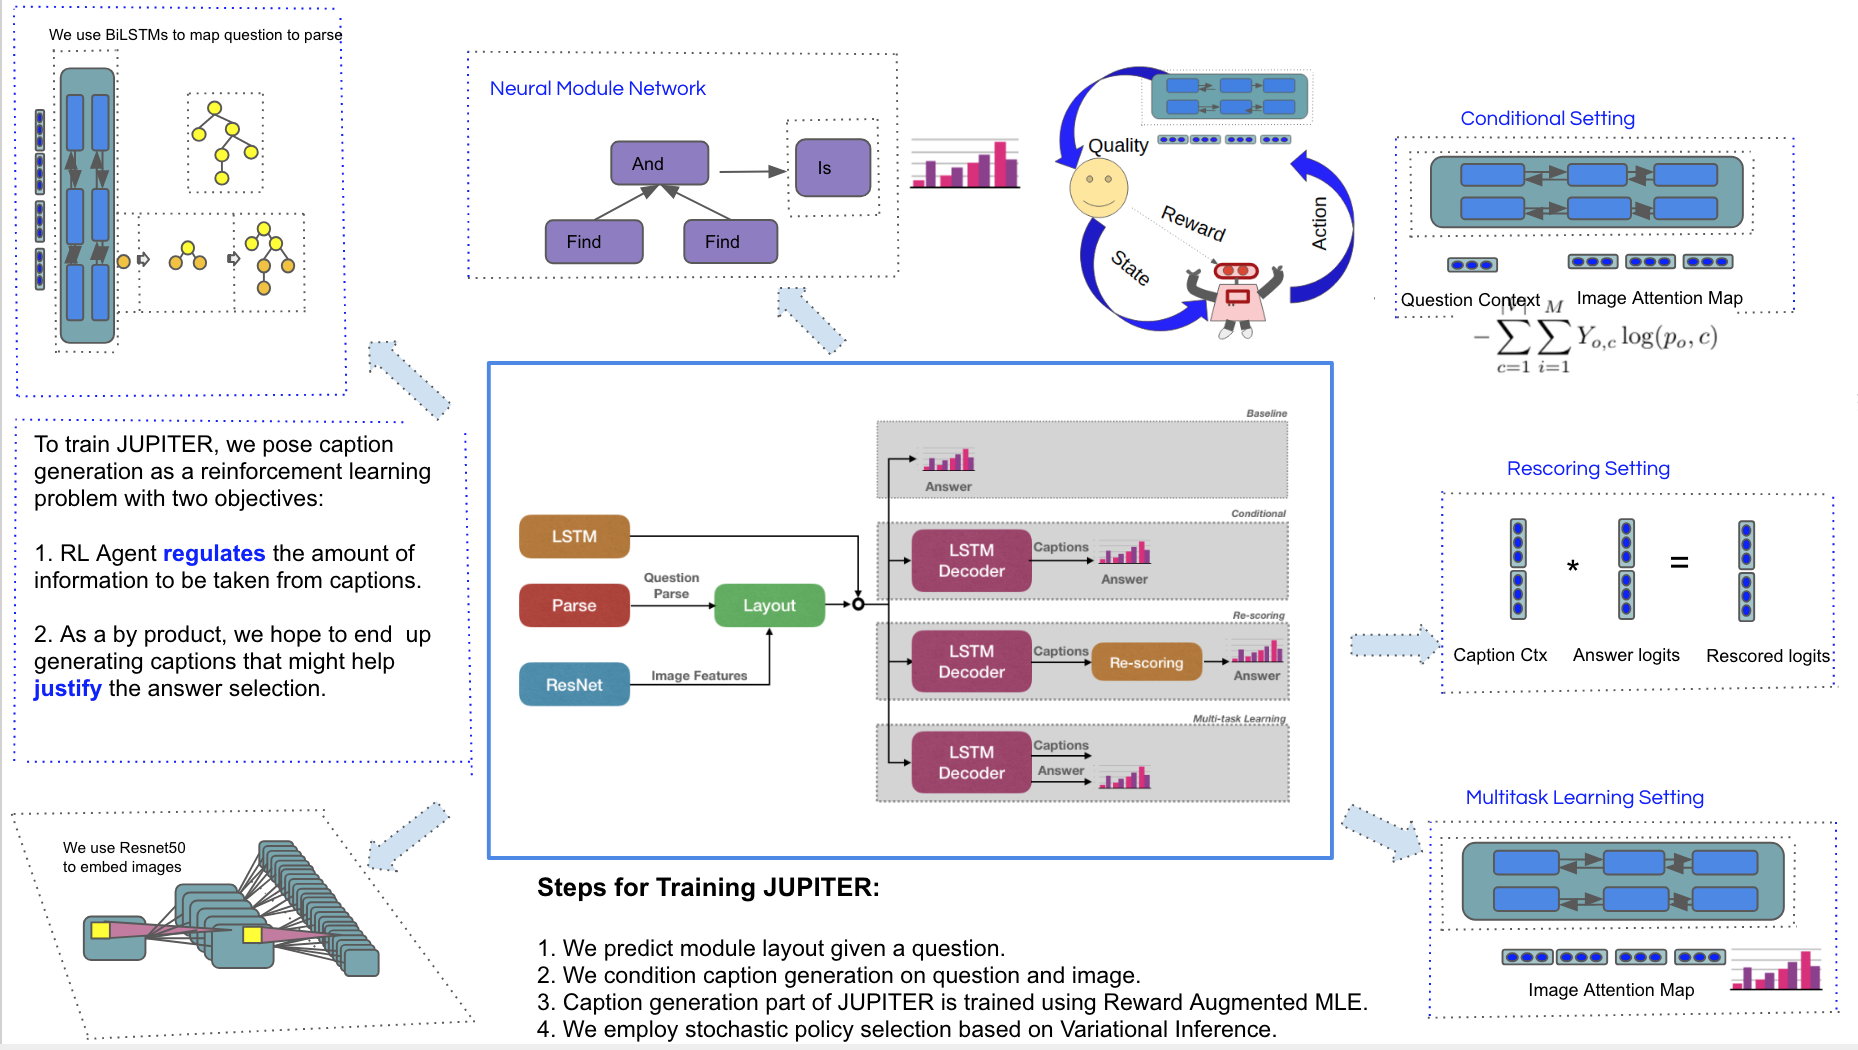
\includegraphics[scale=0.44, frame]{images/jupiter.png}
    \caption{Justification by Pointwise combination of Image and Text based on Expected Rewards}
    \label{fig:jupiter}
\end{figure}
    
    
\subsubsection{Learning}
We denote input question as \textit{Q} and input image as \textit{I}. \textit{L*} denotes the gold layout for \textit{Q} and \textit{C*} is gold caption for \textit{I}. We denote \textit{L} as the layout generated by NMN for \textit{Q}. \textit{C} is caption generated from JUPITER. We denote answer classes by \textit{y} and the correct answer class by \textit{y*}. \textit{T} is the training data samples of type (\textit{I, Q, y*}). Next, we describe the objective function for each extension in detail. 
\begin{itemize}
\item \textit{Multitask Learning}: We use a two-part objective function for multitask learning. The first part is generating  captions from the input and the second is generating answer logits from the input and the generated NMN layout. \\
\begin{equation}
    L(\theta) = \sum_{(I, Q, y*) \in T} logP_\theta(y | I, Q, L) + logP_\theta(C | I, Q)
\end{equation}
 
\item \textit{Conditional Generation}: This extension uses a similar objective function. However, we generate answer logits from the input, generated NMN layout as well as the generated captions.
\begin{equation}
    L(\theta) = \sum_{(I, Q, y*) \in T} logP_\theta(y | I, Q, L, C) + logP_\theta(C | I, Q)
\end{equation}

\item \textit{Re-weighting}: This extension uses a similar objective as conditioned generation. Further, for re-weighting we define new answer logits \textit{y'}. 
\begin{equation}
    y' = C_{T}  y
\end{equation}
where, C$_{T}$ is the final hidden state of generated caption, and y is the previous answer logits. The updated objective function is: 
\begin{equation}
    L(\theta) = \sum_{(I, Q, y*) \in T} logP_\theta(y' | I, Q, L, C) + logP_\theta(C | I, Q)
\end{equation}

\item \textit{Reinforcement Learning}: The agent transitions between generating next word in the caption and generating final answer. The agent receives minibatch VQA accuracy as its reward. The Baseline we use to stabilize the training and  the expected reward of our agent respectively are expressed as 

\begin{equation}
    L_{baseline}(\theta) = \sum_{(I, Q, y*) \in T} logP_\theta(y | I, Q, L, C) 
\end{equation}



\iffalse
\begin{equation}
   Reward = \sum_{n=0}^{N} ( r_n) 
\end{equation}

where N is the length of captions.
\fi

\end{itemize}
We use cross-entropy loss to train the model. We jointly train our captions module in JUPITER alongside NMN, which learns a question layout \textit{L}. 

section{Dataset and Input Modalities}
VQA dataset by \cite{AntolALMBZP15} has 265016 images, 614163
questions.  The dataset consists of  82,783 training, 40,504 validation, and 40,775 test images. Each image has 3 questions on average and 10 ground truth answers. Questions as well as answers are open ended, accounting for a more real-world scenario. The questions are rich in a way, as the require the model to have complex reasoning and understanding abilities.


\section{Results and Discussion}

\iffalse
 When presenting your results, try to follow the same sequence as you specified in the introduction of the Experimental Setup. If you stated 3 research questions, then it would be best to have 3 sub-sections in the Results and Discussion, one for each research question. Present in tables and/or figures your experimental results. It is not enough just to list the results you need to discuss them – what do they mean, what implications they have, how
should they be interpreted in the broader context. If you want to make your results more convincing, where possible, include statistical tests to demonstrate the statistical significance of your findings. You should also include a discussion (if possible, with examples and figures) of the failure cases of the baseline models.
\fi



\begin{figure} [h]
    \centering
    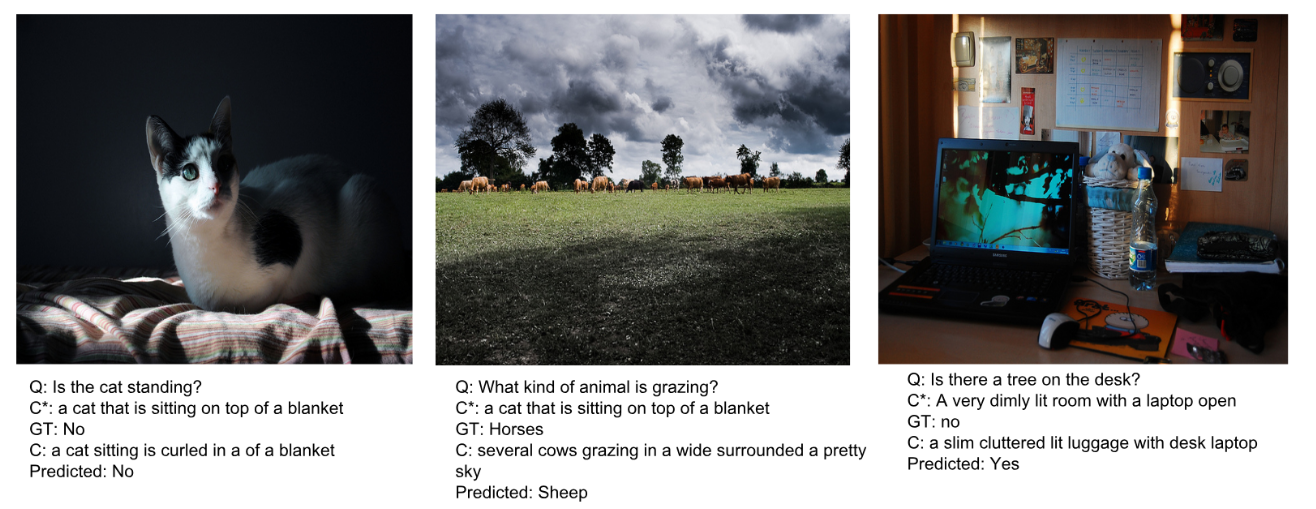
\includegraphics[scale=0.3]{images/captions.png}
    \caption{Qualitative Analysis from JUPITER: left image depicts a scenario where generating caption helped the model in selection of the right answer. Image in the center depicts a scenario where captions end up confusing the model. Image in the right most highlights an interesting scenario where the generated caption seems irrelevant.}
    \label{fig:jupiter_qualitative}
\end{figure}
In this section, we discuss the results from our proposed approaches viz. JUPITER, VENUS and MARS, and compare them against our baselines. Table \ref{results_table} consolidates the results of our experiments. To better understand the performance of these models, we report the performance across different answer categories namely, Number, Yes/No and Other. The overall best baseline model for VQA is NMN by \cite{HuARDS17}.

%In this section, we discuss the results of our proposed approaches in comparison to our baseline models on VQA. 
%We first discuss the baseline results for each of the proposed approach domains. For a better understanding of the models performance, we provide the results by splitting the category of answers into number, yes/no and other type.  The final baseline that we aim to improve over is the one set by module networks. 
section{Results: Baseline Models}
The input to our baseline models is the image and the question. We do not use any external knowledge. Our results show that the baseline models have highest accuracy on the Yes/No questions. However, the Number type questions often require deeper understanding of the image, and so our baselines have lowest performance on them. Humans tend to have low agreement for Yes/No questions. We attribute this to question ambiguity or missing information in the image.It has to be noted that our implementation of the NMN baseline achieves better scores compared to the open source original implementation. This can be attributed to the presence of additional modules in our implementation, specifically OR, COUNT, FILTER, and EXIST modules.

%Comparing across our baselines, NMN outperforms the rest. We believe this is since the model explicitly handles compositionality, providing better generalizability. Amongst the fusion baselines, the RNN performs worse than the VED baseline. We believe this is because VED captures latent representations which are more useful for VQA. 


%Also, our implementation of the NMN baseline is much better than the scores on the original implementation repository. The incorporation of modules - OR, COUNT, FILTER, and EXIST as mentioned in the paper helped generate layouts which were more valid, therefore our implementation was better. 
%The baselines all input only the question and the image, with no addition of external knowledge. Comparing across the three baselines, we see that the NMN is the best baseline we can get for VQA. 



%Question Type:  number Accuracy: 26.352015732546707
%Question Type:  yes/no Accuracy: 64.48818031885652
%Question Type:  other Accuracy: 31.55374946530223
%43.226183422213445 overall


%Question Type:  number Accuracy: 23.310390036053754
%Question Type:  other Accuracy: 26.649336974762264
%Question Type:  yes/no Accuracy: 63.936228697086314
%40.18450852590691 overall

\begin{table}[!h]
\centering
\small
%\scriptsize
\begin{tabular}{@{}lllccc@{}}
%\toprule
%                      & &\textbf{Accuracy(\%)}                                      \\ 
\toprule
                      
{ \textbf{Model}}  & {\textbf{{System}}} & {\textbf{{Input}}}    & \textbf{{Number}}             & \textbf{{Yes/No}}               & \textbf{{Other}}                \\ \midrule
Human & Best & Image + Question & 83.39   & 95.77      &   72.67    \\
Human & Worst & Image + Question  & 65.28          &    46.52   & 78.02      \\ \midrule
NMN  & Baseline (Replicated)                      & Image + Question           &            23.31	         &           63.93          &          	26.65              \\
NMN  & Baseline (Our implementation)                      & Image + Question           &            26.35	         &           64.49          &          	31.55              \\
RNN  & Baseline                    & Image + Question           &    19.34                 &    57.82                 &          17.77           \\
VED & Baseline                      & Image + Question             &     17.76                 &     58.00                &        10.43              \\ \midrule
RNN  &          MARS           & Image + Question + Caption* &                23.09      &       57.88               &     18.22                 \\



RNN   &          MARS          & Question + Caption*        &     21.72                 &             57.95         &      21.59                \\




VED   &        VENUS        & Image + Question + Caption* &   19.25                   &     57.83                 &      10.10                \\

VED   &        VENUS          & Question + Caption*        &            18.13          &        58.10              &        10.33 \\ 
\midrule
%NMN  & Conditional         & Image + Question + Caption &  & & \\
%NMN  & Rescore             & Image + Question + Caption & 27.48 & 65.8  & 32.2 \\
%NMN  & Multitask          & Image + Question + Caption &  & & \\
NMN  & M-Hybrid            & Image + Question + Caption &     26.31                 &       	64.27	            &      30.43                  \\
NMN  & C-Hybrid           & Image + Question + Caption & 27.48 & 65.8& 	32.2\\ 	

NMN & JUPITER     & Image + Question + Caption &  32.82                 &       	67.95	            &      33.15                   \\\bottomrule
\end{tabular}
\caption{Results from human, baselines and proposed approaches. * denotes systems that employ Gold captions}
\label{results_table}
\end{table}

section{Results: Proposed Models}
Looking at the objective evaluation results from table \ref{results_table}, it is clear that incorporating captions leads to improvements across the approaches. This result empirically validates our hypothesis related to captions: Captions help VQA. To understand the extent of this, we have also performed ablation analysis wherein we have used just captions to answer the question ignoring the input image. Surprisingly, systems built in this fashion seem to perform better than our baselines. This leads to an interesting observation: \textit{Captions seem to contain supplementary and in some cases complementary information to the images themselves}. However, we acknowledge that proving such hypothesis would require additional experimentation. For instance, it would be interesting to perform similar ablation analyses employing computationally more powerful frameworks such as attention as baselines or adding more visual information such as ground truth bounding boxes. It is also interesting to note that the proposed approaches achieve better scores compared against the \textit{worst} human performance in Yes/No category.

Our approach JUPITER outperforms all other approaches across all the categories. In addition, within the models employing module networks, the system employing reinforcement learning outperforms other approaches. This is in line with our hypothesis related to Reward Augmented Maximum Likelihood and raises interesting questions related to \textit{comparison between supervised approaches such as Maximum Likelihood and their reward based reinforcement counterparts}. It would be interesting to perform a much larger scale evaluation comprehensively comparing the effectiveness of these approaches in the context of downstream tasks. In figure \ref{fig:jupiter_qualitative}, we present some scenarios that highlight the way captions get utilized for answering question about the corresponding images.





